\section{Simulated Duration and Cutoff Comparison}
\label{sec:simulated-duration-cutoff-comparison}

Figs.~\ref{fig:simulated-duration-cutoff-5us}--
\ref{fig:simulated-duration-cutoff-60us} compare two-dimensional simulated
spectroscopy maps for matched echo-root-Lorentzian and root-Lorentzian pulses.
Each figure fixes the total duration at $L=5$, 20, or $60~\mu\mathrm{s}$;
the columns use relative endpoint cutoffs $c=0.010$, 0.007, and 0.002.  The
upper row is the echo protocol and the lower row is the corresponding pulse
without the central phase inversion.  All panels use the same detuning,
peak-Rabi-frequency, and color scales so that changes between protocols and
cutoffs can be compared directly.

These preliminary maps are generated with the two-level Lindblad model of
Sec.~\ref{sec:numerical-model}.  They use the q1 measurement-linked values
$T_1=\MeasuredTOne~\mu\mathrm{s}$ and
$T_\phi=\EffectiveTPhi~\mu\mathrm{s}$, corresponding to
$T_{2,\mathrm{eff}}=\EffectiveTTwo~\mu\mathrm{s}$.  The maps span
$\Delta/2\pi=-1$ to $1~\mathrm{MHz}$ and
$\Omega_0/2\pi=0$ to $50~\mathrm{MHz}$.  The generalized-Lorentzian exponent
is $n=1/2$, and the endpoint cutoff is imposed at fixed total duration using
Eq.~\eqref{eq:tau-from-cutoff}.  The nonuniform integration grid resolves the
narrow pulse center and contains 1600 fourth-order Runge--Kutta steps per
pulse half.

\clearpage
\begin{figure}[t]
    \centering
    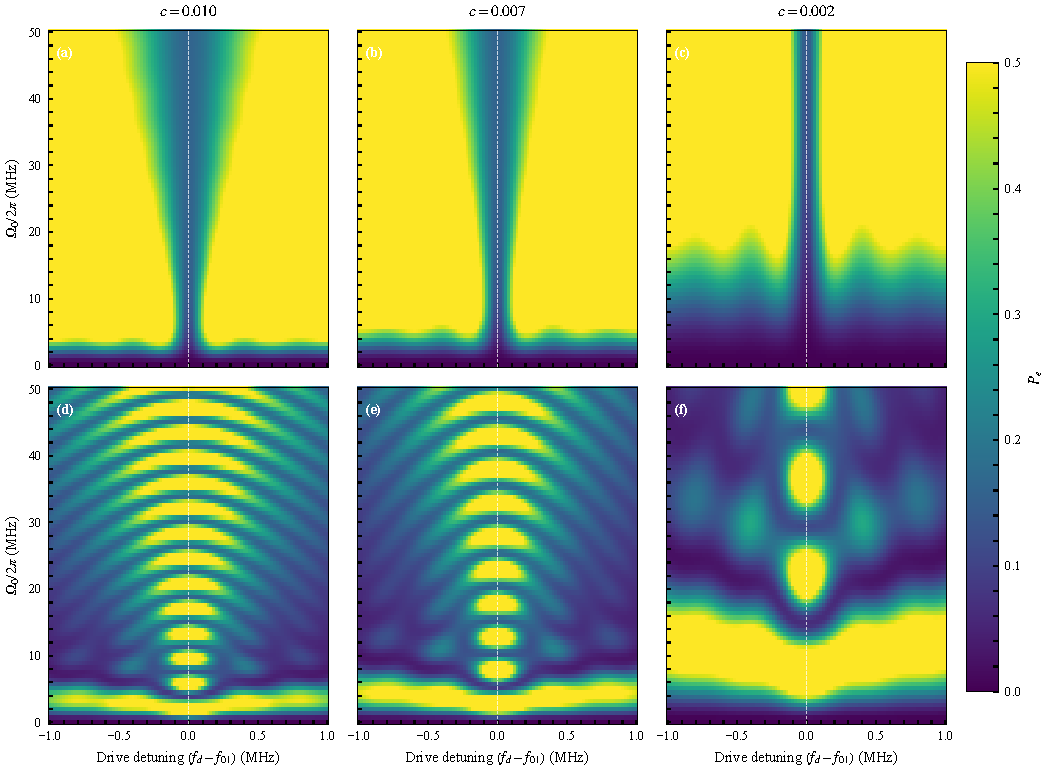
\includegraphics[width=0.98\textwidth]{../figures/paper/09_simulated_echo_lorentzian_5us.pdf}
    \caption{Simulated cutoff comparison for $L=5~\mu\mathrm{s}$.  The upper
    row shows echo-root-Lorentzian spectroscopy and the lower row shows the
    matched root-Lorentzian protocol.  Columns correspond to $c=0.010$,
    0.007, and 0.002.  Every panel displays final excited-state probability
    over the same detuning and peak-Rabi-frequency grid.}
    \label{fig:simulated-duration-cutoff-5us}
\end{figure}
\clearpage

\begin{figure}[t]
    \centering
    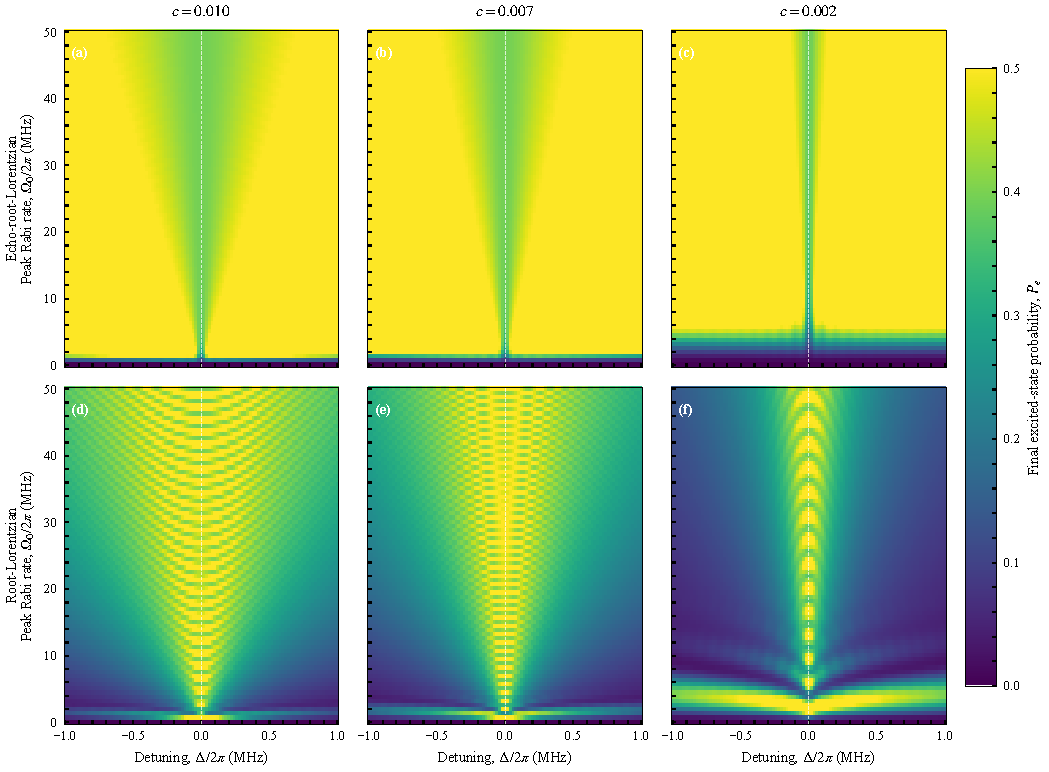
\includegraphics[width=0.98\textwidth]{../figures/paper/09_simulated_echo_lorentzian_20us.pdf}
    \caption{Simulated cutoff comparison for $L=20~\mu\mathrm{s}$, using the
    same layout, axes, color scale, and model parameters as
    Fig.~\ref{fig:simulated-duration-cutoff-5us}.}
    \label{fig:simulated-duration-cutoff-20us}
\end{figure}
\clearpage

\begin{figure}[t]
    \centering
    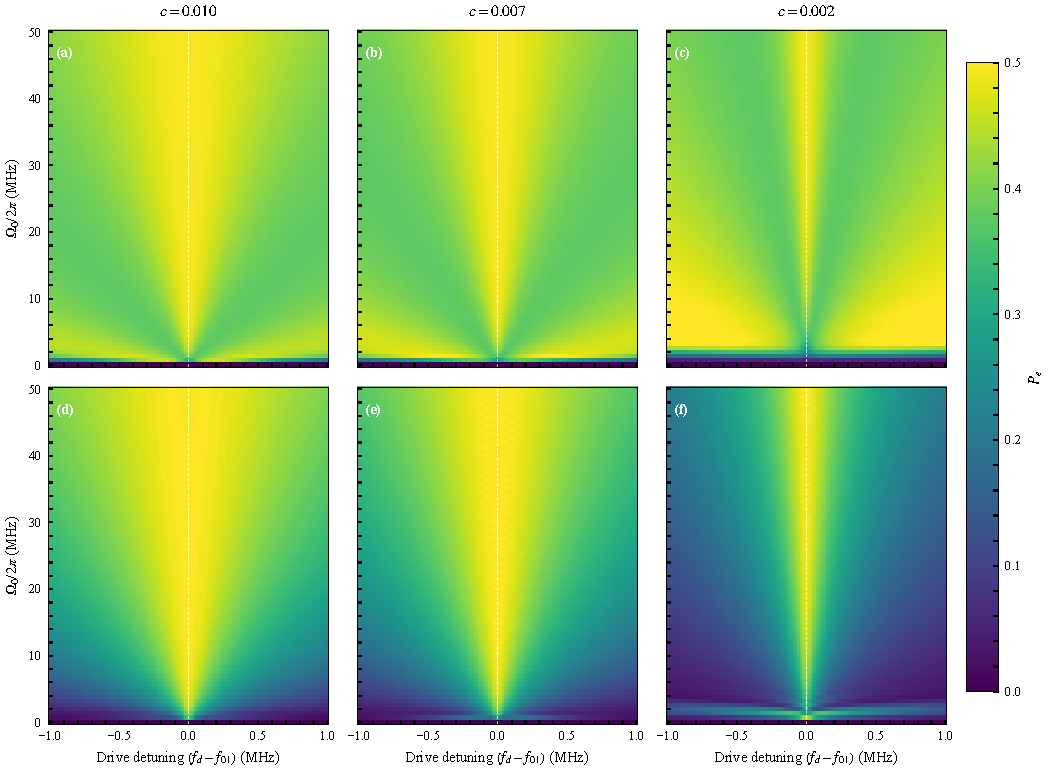
\includegraphics[width=0.98\textwidth]{../figures/paper/09_simulated_echo_lorentzian_60us.pdf}
    \caption{Simulated cutoff comparison for $L=60~\mu\mathrm{s}$, using the
    same layout, axes, color scale, and model parameters as
    Fig.~\ref{fig:simulated-duration-cutoff-5us}.}
    \label{fig:simulated-duration-cutoff-60us}
\end{figure}
\clearpage

\FloatBarrier
